\section{Méthode de Newton}

\subsection{Principe de la méthode de Newton}
La méthode de Newton consiste à \guillemets{linéariser} la fonction $f$ autour d'un valeur $u_0$; on va approximer la fonction par sa tangente et chercher un zéro $u_1$ de cette droite (qui est la \guillemets{linéarisation} de la fonction). On recommence le procédé avec la valeur $u_1$ et ainsi de suite autant de fois que nécessaire. On obtient alors une suite $(u_n)_{n\in \N}$ qui sont les zéros des tangentes successives et qui \guillemets{normalement} converge vers un zéro de $f$.

\medskip
Soit $f:[a,b] \to \R$ une fonction dérivable et $u_0 \in[a,b]$.
On appelle $(u_1,0)$ l'intersection de
la tangente au graphe de $f$ en $(u_0,f(u_0))$ avec l'axe des abscisses.
Si $u_1 \in[a,b]$ alors on recommence l'opération avec la tangente au point d'abscisse $u_1$.
Ce processus conduit à la définition d'une suite récurrente :
$$u_0 \in [a,b] \qquad \text{ et } \qquad u_{n+1} = u_n - \frac{f(u_n)}{f'(u_n)}.$$


En effet, la tangente au graphe de $f$ au point d'abscisse $u_n$ est donnée par la fonction
$$d(x) = f'(u_n)(x-u_n)+f(u_n)$$

\vspace{-4mm}
 Il est facile de déterminer que :

\vspace{-4mm}
$$d(x)=0\ssi[3] 0=f'(u_n)(x-u_n)+f(u_n) \ssi[3]  x=u_n - \frac{f(u_n)}{f'(u_n)}$$

Cette suite converge, sous certaine conditions, vers un zéro de la fonction $f$.

\begin{center}
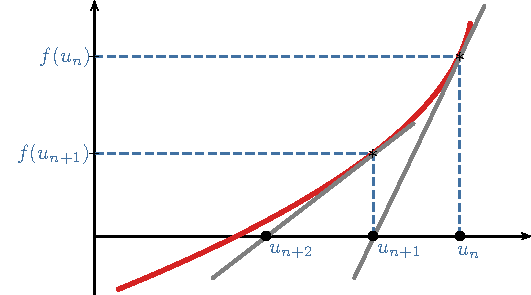
\includegraphics[scale=1]{Chapitre_3_analyse_numerique/figures/fig_6/fig_6.pdf}

\smallskip
\begin{minipage}{0.8\textwidth}
\begin{center}
\textit{\small Les zéros des tangentes forment une suite convergeant vers un zéro de $f$. }
\end{center}
\end{minipage}
\end{center}


\medskip
Lorsque la méthode est applicable, elle est d'une redoutable efficacité. Mais pour que la suite $(u_n)_{n\in \N}$ converge il faut, entre autres conditions, que le point de départ de l'itération ne soit pas trop loin d'un zéro de la fonction. La méthode exige donc de connaître une \guillemets{approximation} de la valeur cherchée.

\medskip
Le résultat suivant, admis sans démonstration, donne les conditions suffisantes pour que la suite converge : 


\begin{theoreme}[\small \textit{convergence de Newton}]\label{convergence_newton}
Soit $f:]a,b[ \to \R$ une fonction deux fois dérivable dont la deuxième dérivée est continue. \\
Si $c\in]a;b[$ est une racine de la fonction $f$ et que $f'(c)\neq 0$, alors il existe $L\in\R$ tel que la suite 
$$u_{n+1}=u_n - \frac{f(u_n)}{f'(u_n)}$$
converge vers $c$ pour tout $u_0\in[c-L;c+L]$.
\end{theoreme}

\begin{minipage}[t][][b]{0.6\textwidth}
Le théorème \ref*{convergence_newton} donne les conditions sur la fonction $f$ pour que la méthode de Newton converge si le point de départ n'est pas trop loin du zéro cherché.

\medskip
Bien que le théorème affirme de l'existence d'un intervalle de convergence, il ne fournit pas d'information sur la longueur de cet intervalle. La longueur de l'intervalle peut-être très petite, et il s'avère parfois utile de recourir à d'autres méthodes pour avoir une première estimation d'un zéro.

\medskip
L'exemple ci-contre montre la méthode de Newton appliquée à la fonction $f$ donnée par :
$$f(x)=\frac{x^3-6x^2+6x+24}{4}$$ 
\end{minipage}\hspace{5mm}\begin{minipage}[t][][b]{0.4\textwidth}
\begin{center}
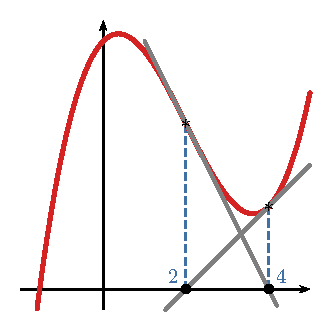
\includegraphics[scale=1]{Chapitre_3_analyse_numerique/figures/fig_7/fig_7.pdf}

\textit{\small La méthode de Newton échoue si $u_0=2$. }
\end{center}
\end{minipage}

\bigskip
Cette fonction possède un zéro en $x\simeq -1,54$, mais si nous initions la méthode avec $u_0=2$ alors la suite qui en résulte oscille entre les valeur $2$ et $4$.

%---------------------------------------------------------------
\subsection{Cas particulier : Calcul de $\sqrt{a}$}

Si on cherche à calculer $\sqrt{a}$, on peut poser $f(x)=x^2-a$ et $f'(x)=2x$. La suite issue de la méthode de Newton pour cette fonction est déterminée par $u_0>0$ et la relation de récurrence : $$u_{n+1} = u_n - \frac{u_n^2-a}{2u_n}$$
Cette suite s'appelle \textbf{suite de Héron}\footnote{Héron d'Alexandrie, mathématicien grec du 1\up{er} siècle après J.C., est connu pour sa formule permettant de calculer l'aire d'un triangle en utilisant la longueur de ses côtés. Cette formule nécessite néanmoins de calculer une racine carrée.} et la proposition \ref*{prop:heron} ci-dessous montre qu'elle converge vers $\sqrt{a}$.


%\begin{exstheorie}
%\begin{enumerate}[label=\textbf{E\thechapter.\arabic*},itemsep=2mm]\setcounter{enumi}{11}
%\item\label{alternative:Heron} Démontrer que la suite de Héron peut s'écrire :  $$u_{n+1} = \frac12 \left(u_n+\frac{a}{u_n}\right)\;$$ et que $u_n\geqslant 0 \eh[2] \forall n\in \N$ (pour  $a,u_0>0$). 
%\end{enumerate}
%\end{exstheorie}




\bigskip
\begin{proposition}
\label{prop:heron}
Pour $a>0$, la suite de Héron définie par $u_{n+1} = u_n - \frac{u_n^2-a}{2u_n}$
 converge vers $\sqrt{a}$ pour tout $u_0>0$.
\end{proposition}

%\textit{Démonstration :}
\begin{demonstration}
\medskip
Soit $u_0>0.$ La suite de Héron peut s'écrire $u_{n+1} = \frac12 \left(u_n+\frac{a}{u_n}\right)$ {\small (voir exercice \ref*{alternative:Heron})}.

\smallskip
Commençons par montrer que $u_n^2 \geqslant a$ pour $n\geqslant 0$. En effet :

$$u_{n+1}^2-a = \frac14 \left(\frac{u_n^2 + a}{u_n}\right)^2 - a = \frac{1}{4u_n^2}(u_n^4-2au_n^2+a^2)=\frac14 \frac{(u_n^2-a)^2}{u_n^2}\geqslant 0$$

Donc $u_{n+1}^2 - a \geqslant 0$ et par conséquent $u_{n}^2 \geqslant a$ pour tout $n\geqslant 0$.

\medskip
Montrons maintenant que $(u_n)_{n\ge1}$ est une suite décroissante. Nous avons :

$$\frac{u_{n+1}}{u_n} = \frac12 \left(1+\frac{a}{u_n^2}\right)$$

\smallskip
et pour $n\geqslant 0$, nous savons que $u_n^2 \geqslant a$ (donc $\frac{a}{u_n^2}\leqslant 1$). Il suit que $\frac{u_{n+1}}{u_n} \leqslant 1$ pour tout $n\leqslant 0$.

\medskip
La suite $(u_n)_{n\ge0}$ est donc décroissante et comme $u_n\geqslant 0$ {\small (voir exercice \ref*{alternative:Heron})} pour tout $n\geqslant 0$, alors la suite est également minorée par $0$. Donc elle converge.\clearpage

\medskip
Notons $\ell$ la limite de la suite $(u_n)_{n\in\N}$. Alors :

\smallskip
$$ u_{n+1} = \frac12 \left(u_n+\frac{a}{u_n}\right) \eh{2}\Rightarrow\eh{2}
 \limn{+\infty}{u_{n+1}}= \limn{+\infty}{\frac12 \left(u_n+\frac{a}{u_n}\right)} \eh{2}\Rightarrow\eh{2} \ell = \frac12 \left(\ell+\frac{a}{\ell}\right)$$ 

On trouve alors facilement que  $\ell^2=a$ et comme les termes de la suites sont positifs on a $\ell = \sqrt{a}$.

\vspace{-3mm}
\hfill $\blacksquare$
\end{demonstration}



\bigskip
\begin{boxexstheorieligne}
\begin{enumerate}[label=\textbf{E\thechapter.\arabic*},itemsep=2mm,resume=refexercices]
\item\label{alternative:Heron} Démontrer que la suite de Héron peut s'écrire :  $$u_{n+1} = \frac12 \left(u_n+\frac{a}{u_n}\right)\;$$ et que $u_n\geqslant 0 \eh{2} \forall n\in \N$ (pour  $a,u_0>0$). 
\item Calculer à la main et sans logiciel une approximation de $\sqrt{2}$ en effectuant 4 itérations de la méthode de Newton avec comme point de départ la valeur $u_0=1$.\\ Combien de décimales sont correctes dans cette approximation?
\item Comparer les résultats de l'exercice précédent avec le résultat de l'exercice \ref*{dicho_racine_2}.\\ Que concluez-vous?
\item Écrire un programme en Python d'une fonction \comp{racine\_carree(a\!;d\!;n)} qui calcule la racine de la valeur \comp{a} en utilisant la suite de Héron. 
\begin{itemize}
\item \comp{d} est la valeur de départ de l'itération,
\item \comp{n} est le nombre d'itérations désirés,
\item la fonction renvoie la valeur estimée du zéro à chaque étape.
\end{itemize}
\item Peut-on appliquer la méthode de Newton à la fonction $\sqrt[3]{x}$ ?
\end{enumerate}
\end{boxexstheorieligne}
\clearpage






